\chapter{AMQP Workflow Orchestration}\label{sec:amqp-workflow-orch}



\section{Overview}

A message queue that supports the AMQP protocol is used to maintain state for \cxoneflow
workflows.  The schema for the exchanges and queues is depicted in Figure \ref{fig:amqp-schema}.
The \texttt{Scan In} exchange is the entrypoint for all workflow state messages.  It is possible
to bind custom topic exchanges and create custom queues to augment or replace some of the
workflows.


\begin{figure}[h]
    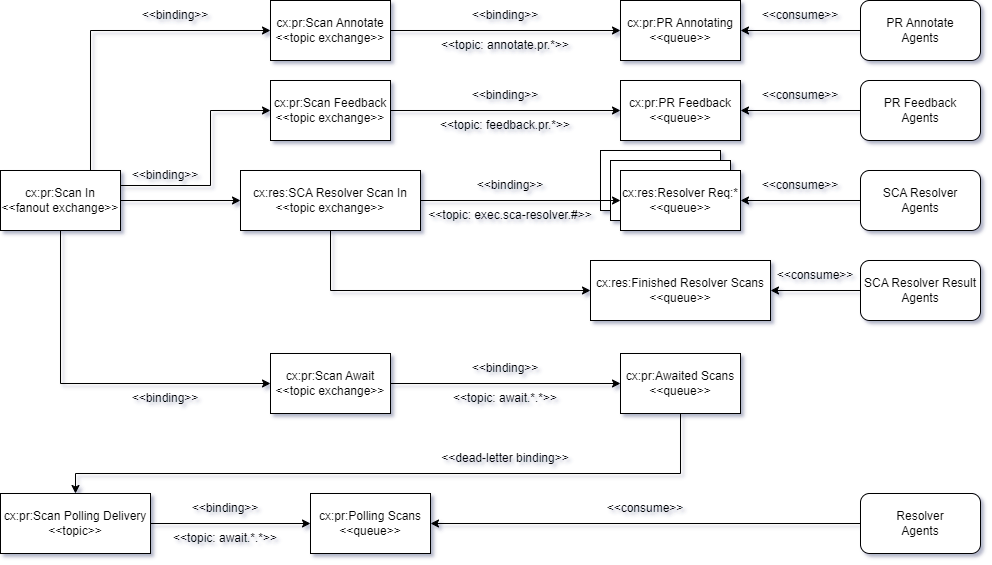
\includegraphics[width=\textwidth]{graphics/cxoneflow-diagrams-Queue.png}
    \caption{AMQP Schema for \cxoneflow}
    \label{fig:amqp-schema}
\end{figure}


\noindent\\Upon startup, each \cxoneflow instance will configure the exchange/queue schema.  An
internal instance of RabbitMQ runs inside the \cxoneflow container to orchestrate
workflows for the container instance.  If an AMQP connection configuration, described in
Section \ref{sec:amqp-element}, is not provided then the local RabbitMQ instance is
used.  When the container is exited, all persisted workflow state information in the local
RabbitMQ instance is lost.  To persist workflow state across container restarts, please
refer to Appendix \ref{sec:high-availability} to deploy \cxoneflow in a
high-availability configuration.

\section{Message Topic Format}

Messages enqueued via the \texttt{Scan In} exchange will have a topic in the format of:

\begin{code}{}{}{}
<scan state>.<workflow>.<service moniker>
\end{code}

\noindent\\Current scan states are:

\begin{itemize}
    \item await
    \item feedback
    \item annotate
\end{itemize}

\noindent\\The \texttt{Scan In} exchange is a fanout exchange that is bound to several topic
exchanges.  The topic for the message submitted to the \texttt{Scan In} exchange is used to
route the message by each bound topic exchange.

\noindent\\For customization purposes, other topic
exchanges may be bound to the \texttt{Scan In} exchange.\footnote{Integration concepts
using AMQP topic exchanges are beyond the scope of this manual.} When a \cxoneflow instance starts,
any customized bindings to the \texttt{Scan In} exchange are not modified.


\noindent\\The \texttt{moniker} segment of the topic is set to the value of the
SCM configurations \texttt{service-name} element as described in
Section \ref{sec:scm-block-element}.

\subsection{The \texttt{await} Scan State}

Messages with the scan state segment of the topic set to \texttt{await} can have the following
values in the workflow segment:

\begin{itemize}
    \item pr
    \item push
\end{itemize}

\noindent\\The \cxoneflow agents send this message when a scan is started.  This begins
the workflow that monitors the state of the scan to detect when the scan finishes
or fails before beginning the next workflow.


\subsection{The \texttt{annotate} Scan State}

Messages with the scan state segment of the topic set to \texttt{annotate} can have the following
values in the workflow segment:

\begin{itemize}
    \item pr
\end{itemize}

\noindent\\The \texttt{annotate} state is used by the workflow to note the status of the
scan.  Please refer to Part \ref{part:feedback-workflows} for details about each supported
workflow.


\subsection{The \texttt{feedback} Scan State}

Messages with the scan state segment of the topic set to \texttt{feedback} can have the following
values in the workflow segment:

\begin{itemize}
    \item pr
\end{itemize}

\noindent\\The \texttt{feedback} state is used by the workflow to map scan result data to
a feedback method appropriate for the scan type workflow.  
Please refer to Part \ref{part:feedback-workflows} for details about each supported workflow.
